\section{Aircraft emissions}
\label{emissions}
Aircraft propulsion systems provide the essential driving force component to enable powerful and efficient flight. In modern commercial aviation, responsible for \textasciitilde88\% of global aviation fuel usage \cite{Gossling2020}, it is commonplace to use a gas turbine propulsion system operating on kerosene-based jet fuel. Aviation's environmental impact stems from the emission and dispersion of chemically and radiatively active substances that are generated during jet fuel combustion. This section details the emissions generation process and the modelling methods implemented to estimate emissions based on aircraft performance calculations and the determination of fuel consumption.

\subsection{The generation of aircraft emissions}
The widespread usage of kerosene-based jet fuels stems from the need to satisfy strict power-to-weight and safety requirements demanded by commercial aircraft; this is because kerosene has an exceptionally high energy density and wide operating temperature range at a low financial cost, compared with alternative fuel types \cite{Hemighaus2007, USDOE_2020}. The stoichiometric combustion of kerosene with air, required to generate thrust, does however generate a number of chemically- and radiatively-active emission species which are emitted from the aircraft into its wake. These aircraft emissions interact with the surrounding atmosphere, perturbing the natural balance of chemistry and contributing to air quality issues and anthropogenic climate change. The mass of emission produced per unit mass of fuel burnt is often referred to as the emission index (EI), measured in grams of emission per kilogram of fuel [g/kg].

\subsubsection{Primary jet fuel combustion products}
The products of jet fuel combustion are often divided into two categories: primary and secondary, alluding to the way in which they are formed inside the aircraft engine. The primary products of jet fuel combustion are carbon dioxide (\ce{CO_2}), water vapour (\ce{H_{2}O}) and, due to fuel impurities, a relatively small amount of sulphur oxides (\ce{SO_x}). These products are generated as a direct result of the combustion reaction that takes place, and hence depends on the carbon-hydrogen-sulphur composition of the fuel. The direct coupling of the production of these species to fuel consumption means that they have a constant EI throughout all phases of flight. Example values based on the typical chemical composition of jet fuel are given in table \ref{primary_EI_tab} \cite{IPCC1999}.

\begin{table}[H]
\centering
\caption{Emission indices estimates for \ce{CO_2}, \ce{H_2O} and \ce{SO_2}, averaged from a range of existing studies testing various aviation fuel types \cite{EUROCONTROL2001}.}
\begin{tabular}{@{}lll@{}}
\toprule
\textbf{\ce{CO_2}} & \textbf{\ce{H_2O}} & \textbf{\ce{SO_2}} \\ \midrule
3.149~g/kg fuel & 1.230~g/kg fuel & 0.84~g/kg fuel \\
\bottomrule
\end{tabular}
\label{primary_EI_tab}
\end{table}

\subsubsection{Secondary jet fuel combustion products}
Further to this, a number of secondary combustion products are generated in the aircraft exhaust, namely oxides of nitrogen (\ce{NO_x} $\equiv$ NO \& \ce{NO_2}), carbon monoxide (CO), unburnt hydrocarbons (HC), particulate matter (PM) and trace levels of volatile organic compounds (VOCs) \cite{Brasseur1998}. These products are termed secondary because their production levels differ depending on the nature of the combustion process and the engine load condition \cite{Deidewig1996}. This means that their EIs are variable throughout flight, depending on aircraft engine type, engine operating conditions, and the atmospheric conditions of the surrounding environment \cite{Dopelheuer2000}.
%IPCC chapter 7 ^
c
\ce{NO_x} emissions originate from the entry of atmospheric nitrogen (\ce{N_2}) into the high temperature combustion chamber. The level of \ce{NO_x} increases with increasing temperature and pressure, as it is coupled to the thermal reaction processes that occur in the primary combustion zone. Therefore, with the assumption of constant polytropic and combustion efficiencies, the emission index of \ce{NO_x} (EI\ce{NO_x}) can be correlated with aircraft fuel flow \cite{Dopelheuer1998, Deidewig1996}. As a result of inefficiencies in the combustion process, products such as CO and HC are formed. In contrast to \ce{NO_x}, these emissions are direct products of incomplete combustion, meaning their concentrations are inversely proportional to combustion efficiency. Since combustion efficiency correlates with thrust for sea level static (SLS) conditions, and thrust correlates with fuel flow, this means that EICO and EIHC decrease with increasing fuel flow. 

PM emissions from aircraft can be categorised by their volatility: non-volatile PM (nvPM) and volatile PM (vPM). The primary source of nvPM present in aircraft exhaust is soot, which constitutes the greatest warming effect of all particles released from aircraft \cite{Gettelman2013}. Soot is generated in the fuel-rich regions of the combustor, where the condensation of unburnt aromatic hydrocarbons takes place, converting low carbon content HC fuel molecules into carbonaceous agglomerates containing millions of carbon atoms \cite{Ebbinghaus2001, Bockhorn1994}. The extent of soot formation therefore depends on the fuel-air-ratio and the mixing processes that take place in the combustor, which vary with combustor design and are influenced by the non-homogeneous flow and temperature fields. Accurate measurements of these parameters are rare, making it very difficult to directly acquire quantitative data on soot emissions. Instead, soot EI can be estimated based on correlation with the so-called smoke number measured in engine certification procedures \cite{Dopelheuer1998}.

The formation of vPM from aircraft largely derives from the emission of sulphur derivatives, lubrication oil and VOCs \cite{Wayson2012}. During combustion, the sulphur content in the fuel is mostly oxidised to sulphur dioxide (\ce{SO_2}), some of which is then further oxidised to sulphuric acid (\ce{H_{2}SO_{4}}) when emitted into the atmosphere. In the presence of sufficient water vapour, sulphate aerosols (\ce{SO_4}) can be generated, which exhibit the largest cooling effect from aircraft PM emissions \cite{IPCC1999}. The sulphate EI is a factor of fuel sulphur content, which varies depending on fuel composition and the specific emissions characteristics of the engine \cite{Schumann2002}. Due to the low volatility of lubricant oil, the emitted oil vapour from aircraft will add to the condensed mass of VOCs and contribute to vPM concentrations. The VOCs produced either from the oxidized fuel fragments or due to the pyrolysis in the combustion chamber can also act as vPM, which may have sufficiently low vapour pressure to allow condensation in the atmosphere, forming a coating on the surface of the nvPM and impacting cloud formation, precipitation and climate \cite{IPCC1999}. The particulate matter emitted near the exit nozzle plane of the combustor consists only of nvPM, but vPM are produced through nucleation and condensation downstream. Thus it is difficult to estimate the total amount of vPM produced within the exhaust plume, as the formation of vPM is dependent on the concentration of sulphates and VOCs present in the exhaust, and the distance from the combustor \cite{Masiol2014}.

% Schumann and Fahey IPCC 1999 chapter 3 ^

% Masiol figure here?

\subsection{Aircraft emissions modelling}
Accurate quantification of aircraft emissions for any given flight requires the calculation of aircraft performance to estimate the total energy consumed, and hence the total fuel burnt throughout the flight duration. With knowledge of fuel flow rates experienced throughout flight, flow rates of aircraft emission species can be deduced based on empirical engine performance datasets and emissions models.

\subsubsection{Fuel burn estimation}
Computational modelling of aircraft performance allows the simulation of aircraft trajectories and the quantification of forces experienced throughout flight, enabling the approximation of thrust and fuel flow across all phases of flight. Aircraft performance models that are prevalent in academia and industry, such as the BADA (Base of Aircraft DAta) method \cite{Nuic2010} and Piano-X \cite{PIANO_X}, approximate aircraft behaviour by coupling a database of aircraft-specific performance datasets to mathematical models to calculate useful flight characteristics, such as fuel flow and fuel burn, at discrete time steps during flight. This iterative approach accounts for the time-varying nature of aircraft properties like mass, speed and heading, thus leading to a more accurate estimate of performance and fuel burn estimation. Further to this, models such as the Aviation Environment Design Tool (AEDT) \cite{AEDT} exist, which carry out four-dimensional (4-D) physics-based simulations of aircraft trajectories at an exceptionally high spatial and temporal resolution, providing highly accurate predictions of fuel consumption and localised emissions impacts. Such tools do however come at the expense of high computational and financial cost, and often require proprietary data that is not in the public domain. An alternative state-of-the-art open-source performance model that has been made available in recent years is the OpenAP model \cite{Sun2020}. This consists of four main components: aircraft and engine properties, kinematic performance and dynamic performance, and utility libraries; and can describe the characteristics of 27 common aircraft and 400 turbofan engines. The authors present a favourable comparison to established methods, matching BADA's fidelity across many characteristics, and exceeding it in several, deeming it a feasible alternative for researchers who do not have access to data and licensing for proprietary models. 

\subsubsection{Calculating aircraft emissions at reference conditions}
Aircraft performance models provide estimates of aviation fuel burn, but to determine the particular chemical speciation of emissions released due to fuel combustion aircraft emissions models must be implemented. As mentioned earlier, the primary combustion products, \ce{CO_2}, \ce{H_2O} and \ce{SO_2}, have a direct relation to the amount of fuel burnt and hence a constant EI for a given fuel composition, with standard estimates provided in table \ref{primary_EI_tab}. Secondary combustion products such as \ce{NO_x}, CO and HC however, largely depend on operational and atmospheric conditions. Empirical relationships between EI and fuel flow for secondary combustion products have been determined at reference operating conditions using engine performance datasets, such as the International Civil Aviation Organisation (ICAO) engine emissions databank \cite{ICAOEEDB}.  This databank was developed for the purpose of engine certification and compliance with landing and take-off (LTO) cycle emissions standards, outlined in ICAO Annex 16 Vol. II \cite{ICAO2008}. Engine test data have been collected at sea-level static (SLS), International Standard Atmosphere (ISA) conditions, for four reference operating conditions (thrust settings) relevant to the LTO cycle: take-off (100\% thrust), climb out (85\%), approach (30\%) and taxi in/out (7\%). For every engine at each of the four LTO modes, a reference fuel flow and corresponding emission index has been derived, allowing emissions to be estimated to a reasonable degree of accuracy for aircraft operating under any of the four modes. An exemplar ICAO EI dataset is provided in table \ref{secondary_EI_tab}.

%As alluded to previously, the primary combustion products, \ce{CO_2}, \ce{H_2O} and \ce{SO_x} have a direct relation to the amount of fuel burnt and hence a constant EI for a given fuel composition, whereas the secondary products largely depend on operational and atmospheric conditions. Emissions of \ce{NO_x}, CO and HC can be correlated with fuel flow, meaning estimation of their emission indices requires knowledge of this relationship across the range of operating conditions experienced throughout flight. 



\begin{table}[H]
\centering
\caption{Example ICAO engine emissions data for Rolls Royce Trent 970-84 engine \cite{ICAOEEDB}.}
\begin{tabular}{lllll}
\hline
 & \textbf{Take-off} & \textbf{Climb out} & \textbf{Approach} & \textbf{Idle} \\ \hline
\textbf{Fuel flow {[}kg/s{]}} & 2.605 & 2.157 & 0.720 & 0.255 \\
\textbf{EI \ce{NO_x} {[}g/kg{]}} & 38.29 & 29.42 & 12.09 & 5.44 \\
\textbf{EI CO {[}g/kg{]}} & 0.32 & 0.31 & 1.16 & 13.38 \\
\textbf{EI HC {[}g/kg{]}} & 0.02 & 0.12 & 0.08 & 0.04 \\ \hline
\label{secondary_EI_tab}
\end{tabular}
\end{table}

\subsubsection{Calculating aircraft emissions at non-reference conditions}
In reality, aircraft spend the majority of flight outside of the LTO vicinity (above 3,000~ft), and the operating conditions and atmospheric conditions vary considerably. To enable the accurate analysis of aircraft emissions outside of reference conditions, a number of emissions modelling methods have been developed. Such methods apply the necessary adjustments and interpolations to the LTO-limited engine performance datasets, to generate more realistic estimates of aircraft emissions across the whole flight profile. SAE International Aerospace Information Report 5715 (AIR5715) \cite{AIR5715} describes a number of methods for calculating aircraft emissions throughout all modes of operation and compares their relative merits. For the primary combustion species, the Fuel Composition method is presented, which determines EI\ce{CO_2}, EI\ce{H_2O} and EI\ce{SO_x} from the proportions of carbon, hydrogen and sulphur in the fuel. The set of methods concerning the estimation of EI\ce{NO_x}, EICO and EIHC include the ICAO reference method, the Boeing fuel flow method 2 (BFFM2), the DLR fuel flow method and the P3T3 method, in order of increasing fidelity. The ICAO reference method serves as the simplest and least accurate approach, computing emissions purely based on the ICAO reference conditions, without applying corrections to account for atmospheric effects at altitude. Therefore, it is only applicable for emissions analysis of aircraft flying in the LTO region.  The remaining methods, BFFM2, DLR and P3T3 can be applied at all aircraft operating conditions, including at cruise, as they apply interpolations to engine performance datasets to determine emissions indices throughout the whole duration of a flight. The BFFM2 method and the DLR method (\ce{NO_x} only) are the mid-tier models, as they provide reasonable estimates of EIs purely from interpolating the EI reference data and applying corrections for atmospheric effects based on ambient meteorological data, aircraft fuel flow and Mach number. The gold standard for modelling of \ce{NO_x}, CO and HC emissions is the P3T3 method, as it utilises detailed thermodynamic modelling data to determine the precise emission indices at any given point throughout flight. Required data includes the combustor inlet temperature (T3), pressure (P3) and the fuel-air ratio (FAR) at both reference and operational conditions, all of which are difficult to obtain without access to proprietary engine-specific performance data, which limits the accessibility of this model to open-access researchers \cite{Brink2020, Dubois2006}.

Figure \ref{BFFM2} shows an example of how EIs are interpolated based on the logarithmic relationship between EI and fuel flow, using the BFFM2 method \cite{Wasiuk2014}. Furthermore, methods are also presented to account for the remaining key emission species, such as the Derivative Factor method \cite{AEDT} used to approximate the EI values for VOCs such as non-methane HC (NMHC) throughout flight and the First Order Approximation method \cite{Wayson2012} used to estimate PM emission indices. The choice of method generally depends on the emission species to be observed, the compromise between modelling resources and data availability, and the level of accuracy required.

\begin{figure}[H]
  \centering
  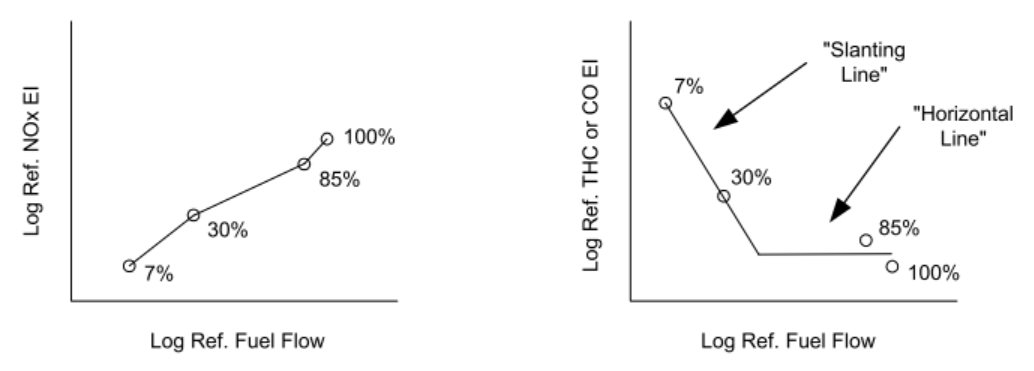
\includegraphics[width=0.9\linewidth]{BFFM2_output_example.png}
  \caption{Example log-log plots of EI against fuel flow at reference conditions, as prescribed by the BFFM2. The percentage values refer to the thrust as a percentage of maximum thrust at SLS conditions \cite{AIR5715}.}
  \label{BFFM2}
\end{figure}

\subsubsection{Emissions inventories and integration into large-scale climate models}
The estimation of aircraft emissions for a specific flight involves the simulation of aircraft performance across the entire flight profile so as to estimate fuel flow and engine operating conditions throughout flight. Knowledge of fuel flows and engine performance characteristics permits the estimation of aircraft emissions, based on the coupling of empirical engine certification data and emissions modelling methods, which interpolate the data to determine the emissions at non-reference conditions. This emissions estimation procedure is commonly carried out on a regional and global scale to determine emissions from a whole range of flights, which are then stored in so-called emissions inventories \cite{Wasiuk2016}. Aircraft emissions inventories collate data from all flights in the desired range and populate three-dimensional (3-D) latitude-longitude-altitude grid cells (e.g. 1\textdegree $\times$ 1\textdegree $\times$ 1000~ft) with total emissions quantities \cite{Paoli2011}. 

Aircraft emissions inventories are utilised to model the atmospheric effects of aviation, using large-scale models that capture the chemistry, physics and dynamics of the Earth-atmosphere system (see section \ref{Climate_modelling} for further detail on climate modelling approaches). Such models allow one to simulate the perturbation to the state of the atmosphere due to an input of emissions and, in turn, provide quantitative indicators that enable modellers to determine the resultant climate impact (e.g. concentrations of key greenhouse gases, aerosol formation and distribution, cloud processes etc.) \cite{Jacobson2005}. O ne underlying issue with this conventional approach to aviation climate modelling is that the use of gridded emissions data inherently assumes the instantaneous dispersion (ID) of emissions into the latitude-longitude-altitude computational grid cell in which they were released \cite{Petry1998}. The dimensions of this grid cell are solely determined by the spatial resolution of the global model, and hence do not serve as an accurate physical representation of emissions dispersion.

In reality, emissions released from aircraft are confined to the aircraft exhaust plume, which inhibits mixing with the surrounding atmosphere for up to a day after emission. Throughout this time, a number of nonlinear chemical and microphysical processes occur, due to the elevated concentrations of emissions species in the plume. These nonlinear plume-scale processes affect the eventual climate response to these emissions, yet most regional and global aviation climate impact studies \cite{Cariolle2009} often neglect the presence of the aircraft exhaust plume and opt for the simplified ID method. The following section explores the dynamical evolution of emissions following their release into ambient air, and discusses modelling approaches present in the literature which can be implemented to represent plume-scale effects in large-scale models. Such modelling is, however, often set aside due to computational issues associated with resolving consistency between the two model resolutions. 


%Throughout history, hydrocarbon fuels have been the dominant fuel source for aviation propulsion purposes, due to their unparalleled energy content and ease of availability.

%The allure towards fossil-based aircraft propulsion throughout the history of commercial aviation has resulted in grave environmental consequences, due to the harmful chemical species emitted into the atmosphere at aircraft cruising altitudes. 

%For an aircraft to achieve and maintain airborne status, it is required that the resistive force due to aerodynamic drag (D) and the gravitational force due to aircraft weight (W) are sufficiently overcome. The necessary driving force required to counteract drag and maintain forward speed is known as thrust (T). The forward speed induces airflow over the aircraft's cambered wings, thus rotating the flow downwards and generating lift (L) to counteract the aircraft weight. These constitute the four fundamental forces of flight \cite{Anderson1999}. The combination of these forces in varying magnitudes determines the trajectory of an aircraft and its instantaneous velocity and acceleration. The performance of an aircraft is highly dependent on the optimisation of the four forces, with structural configuration, material utilisation and payload affecting the aircraft’s weight, balance and stability, and the aircraft geometry affecting aerodynamics and hence influencing the lift and drag forces acting upon it. The thrust force however, is generated by means of a propulsion system. 
%
%\begin{figure}[H]
%  \centering
%  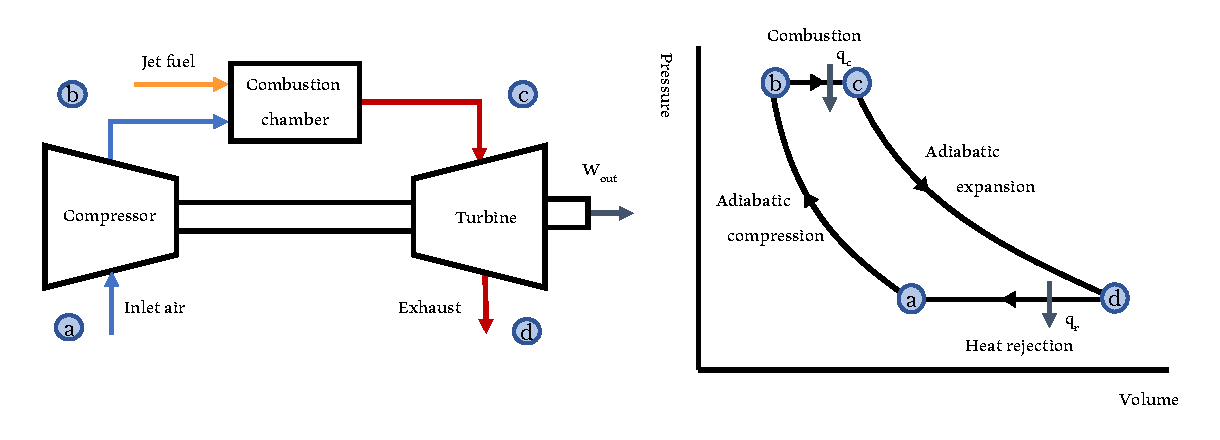
\includegraphics[width=1\linewidth]{Brayton.pdf}
%  \caption{The open-cycle Brayton thermodynamic cycle and its corresponding pressure-volume diagram, adapted from \cite{}.}
%  \label{Brayton}
%\end{figure}
%
%Traditional gas turbine engines, known as turbojet engines, employ the following four point Brayton thermodynamic cycle (see figure \ref{Brayton}): (a--b) the engine ingests oncoming air flow and passes it through a compressor, reducing volume and increasing total pressure; (b--c) the compressed air is mixed with fuel and ignited to cause a combustion reaction, with $q_c$ representing the heat addition to the system; (c--d) the high temperature, high pressure combustion products are passed through a turbine which extracts some energy from the flow to do work ($W_{out}$) to drive the compressor; (d--a) the airflow leaves the engine and is rejected into the atmosphere ($q_r$) at an accelerated rate through the exhaust nozzle. The magnitude of thrust generated by the engine is dependent on the mass of air being accelerated, and the difference in velocity of the air mass through the propulsion system \cite{Oates1989}. The commercial fleet of today primarily use bypass turbofan engines, which have an additional fan installed at the engine inlet. This fan is also powered by the turbine and its purpose is to bypass most of the intake air through the outer duct (often around \textasciitilde90\% according to modern day bypass ratios \cite{}. The addition of a bypass fan serves to increase the mass flow of air being accelerated by the engine, generating additional thrust without the need to burn additional fuel. This leads to a net increase in fuel efficiency of the engine compared to the turbojet equivalent, as the additional thrust generated due to the bypass design outweighs the additional fuel burn required to power the fan \cite{Richter2012}.



